\documentclass{article}

\usepackage{amsmath, amsthm, amssymb}
\usepackage{geometry}
\geometry{margin = 3.0 cm}
\usepackage{float}
\usepackage{algorithm2e}
\usepackage{caption}
\usepackage[]{mcode}
\usepackage{algpseudocode}
\algblockdefx[NAME]{Input}{EndInput}
    [1][]{\textbf{Input:} #1}
    {}

\algblockdefx[NAME]{Output}{EndOutput}
    [1][]{\textbf{Output:} #1}
    {}

\newcommand{\myalg}[2]{\begin{figure}[h]
    { \renewcommand{\figurename}{Algorithm}
\begin{center}
\begin{minipage}{0.6\textwidth}
\hrulefill
\begin{algorithmic}[1]
    #1
\end{algorithmic}
\hrulefill
\end{minipage}
\end{center}
\caption{#2}
}
\end{figure}}

\renewcommand{\l}{\lambda}
\renewcommand{\L}{\Lambda}
\renewcommand{\mod}{~\mathrm{mod}~}
\renewcommand{\div}{~\mathrm{div}~} 
\renewcommand{\vec}[1]{\mathbf{#1}}

\renewcommand{\(}{\left(}
\renewcommand{\)}{\right)}

\newcommand{\dist}{\text{dist}}

\newcommand{\mat}[1]{\begin{pmatrix} #1 \end{pmatrix}}
\newcommand{\room}{\hspace{0.5cm}}
\newcommand{\hl}[1]{\textbf{#1}}
\newcommand{\ceil}[1]{\lceil #1 \rceil}
\newcommand{\floor}[1]{\lfloor #1 \rfloor}
\newcommand{\var}[1]{$\mathtt{#1}$}
\newcommand{\mc}[1]{\mathcal{#1}}
\newcommand{\hot}[1]{\mathcal{O}\(#1\)}
\newcommand{\minimx}[4]{\begin{pmatrix}{#1} & {#2} \\ {#3} & {#4} \end{pmatrix}}

\newcommand{\uin}{u_i^n}
\newcommand{\uinp}{u_i^{n+1}}
\newcommand{\uinm}{u_i^{n-1}}
\newcommand{\uipn}{u_{i+1}^n}
\newcommand{\uimn}{u_{i-1}^n}
\newcommand{\uimnp}{u_{i-1}^{n+1}}
\newcommand{\uipnm}{u_{i+1}^{n-1}}
\newcommand{\uipnp}{u_{i+1}^{n+1}}

\newcommand{\ujn}{u_j^n}
\newcommand{\ujnp}{u_j^{n+1}}
\newcommand{\ujnm}{u_j^{n-1}}
\newcommand{\ujpn}{u_{j+1}^n}
\newcommand{\ujmn}{u_{j-1}^n}
\newcommand{\ujmnp}{u_{j-1}^{n+1}}
\newcommand{\ujpnm}{u_{j+1}^{n-1}}
\newcommand{\ujpnp}{u_{j+1}^{n+1}}

\newcommand{\xin}[1]{{#1}_{i}^n}
\newcommand{\xinp}[1]{{#1}_{t i}^{n+1}}
\newcommand{\xtinm}[1]{{#1}_{t i}^{n-1}}
\newcommand{\xipn}[1]{{#1}_{t i+1}^n}
\newcommand{\ximn}[1]{{#1}_{t i-1}^n}
\newcommand{\ximnp}[1]{{#1}_{t i-1}^{n+1}}
\newcommand{\xipnm}[1]{{#1}_{t i+1}^{n-1}}
\newcommand{\xipnp}[1]{{#1}_{t i+1}^{n+1}}

\newcommand{\yin}[1]{{#1}_{i}^n}
\newcommand{\yinp}[1]{{#1}_{i}^{n+1}}
\newcommand{\ytinm}[1]{{#1}_{i}^{n-1}}
\newcommand{\yipn}[1]{{#1}_{i+1}^n}
\newcommand{\yimn}[1]{{#1}_{i-1}^n}
\newcommand{\yimnp}[1]{{#1}_{i-1}^{n+1}}
\newcommand{\yipnm}[1]{{#1}_{i+1}^{n-1}}
\newcommand{\yipnp}[1]{{#1}_{i+1}^{n+1}}

\newcommand{\vin}{v_i^n}
\newcommand{\vinp}{v_i^{n+1}}
\newcommand{\vinm}{v_i^{n-1}}
\newcommand{\vipn}{v_{i+1}^n}
\newcommand{\vimn}{v_{i-1}^n}
\newcommand{\vimnp}{v_{i-1}^{n+1}}
\newcommand{\vipnm}{v_{i+1}^{n-1}}
\newcommand{\vipnp}{v_{i+1}^{n+1}}

\newcommand{\dt}{\Delta t}
\newcommand{\dx}{\Delta x}
\newcommand{\dxi}{\Delta \xi}
\newcommand{\ctx}{\frac{c\dt}{\dx}}
\newcommand{\half}[1]{\frac{{#1}}{2}}




\newtheorem{lem}{Lemma}

\usepackage{tikz} \usetikzlibrary{shapes}
\usetikzlibrary{arrows}

\tikzset{node distance=3cm, auto}

\begin{document}
\title{Exercise F4a}
\author{Abe Wits (3629538)}
\date{2015/04/15}%TODO the date

\maketitle

\setlength{\parskip}{0.2 cm}
\setlength{\parindent}{0.0 cm}

\section*{Write models 1 and 2 as a system of two first-order PDEs (in time) as discussed in exercise \textbf{SC1}}
We can rewrite $u_{tt} = u_{xxx}$ as;
$$
\begin{cases}
v = u_t\\
v_t = u_{xxx}
\end{cases}
$$

\section*{Describe and implement a boundary-value (BV) technique for both models. For a description of BV we refer to the documents on the web page of this course. Note that different choices can be made for the time-integration part of BV and also for its (extra) final condition at $t=T$}
We have to make our PDEs discrete. We use leapfrog for our time integration and we use the $\hot{(\dx)^2}$ space discretization we derived in SC1;
$$u_t \approx \frac{\uinp - \uinm}{2\dt} \;\;\;\;\mathrm{and}\;\;\;\;v_t \approx \frac{\vinp - \vinm}{2\dt}$$
$$u_{xxx} \approx \frac{-\half{u_{i-2}^n}+\uimn-\uipn+\half{u_{i+2}^n}}{(\dx)^3}$$

We want to construct a system of linear equations that solves our PDE. The equations above can be used to construct linear constraints: we want to enforce that $v=u_t$ and $v_t=u_{xxx}$;
$$v = u_t \approx \frac{\uinp - \uinm}{2\dt}$$
\begin{equation}
\uinp-2\dt\vin-\uinm = 0
\label{eq:uin}
\end{equation}
And similarly:
$$\frac{\vinp - \vinm}{2\dt} \approx v_t = u_{xxx} \approx \frac{-\half{u_{i-2}^n}+\uimn-\uipn+\half{u_{i+2}^n}}{(\dx)^3}$$
\begin{equation}
\vinp-\frac{2\dt}{(\dx)^3}\(-\half{u_{i-2}^n}+\uimn-\uipn+\half{u_{i+2}^n}\)-\vinm = 0
\label{eq:vin}
\end{equation}
In this system we see $\uin$ and $\vin$ as our variables. Let $T = N\dt$, then $n\in\{0,1,\dots,N\}$. Similarly we choose $x_M=x_{max}$ and $x_0=x_{min}$, with $m \in \{0,1,\dots,M\}$. We will handle boundary conditions in the space direction separately for the different models.
Notice that our constraints are invalid if they contain non-existent variables such as $u_i^{N+1}$, $v_i^{N+1}$, $u_i^{-1}$ or $v_i^{-1}$. We do not use such invalid constraints, but add boundary conditions for $n=0$ and $n=N$ instead:
\begin{equation}
u_i^0 = u(x_i, 0)
\label{eq:ui0}
\end{equation}
\begin{equation}
u_i^N = u(x_i, T)
\label{eq:uiN}
\end{equation}
\begin{equation}
v_i^0 = v(x_i, 0)
\label{eq:vi0}
\end{equation}
\begin{equation}
v_i^N = v(x_i, T)
\label{eq:viN}
\end{equation}
The functions $u_0$, $v_0$ (the initial conditions)  and $u_T$, $v_T$ (the final conditions) are different functions for model 1 and model 2.
If all boundary conditions are chosen correctly, the number of constraints is exactly equal to the number of variables. We will write the system in the standard form, $A w = b$, where $A$ is a (known) matrix with all constraints, $b$ is a (known) vector with all the constants from the constraints, and $w$ the (unknown) vector that will contain our solution. We will handle the construction of $A$ and $b$ separately for model 1 and model 2.

\subsection*{Model 1}
We have periodic boundary conditions, so $x_0 = x_{min} = x_{max} = x_M$. Our initial condition is $u(x, 0) = \sin(2\pi x)$ and $v(x, 0) = 0$. For the final condition on $u$ we use the exact solution given, and for $v$ we use its derivative; 
$$u(x,t) = \frac{1}{2} e^{-2 \pi ^{3/2} t} \left(\sin \left(2 \pi  \left(\sqrt{\pi } t+x\right)\right)-e^{4 \pi ^{3/2} t} \sin \left(2 \pi ^{3/2} t-2 \pi  x\right)\right)$$
$$v(x,t) = \pi ^{3/2} e^{-2 \pi ^{3/2} t} \left(-\sin \left(2 \pi  \left(\sqrt{\pi } t+x\right)\right)+\cos \left(2 \pi  \left(\sqrt{\pi } t+x\right)\right)-e^{4 \pi ^{3/2} t} \left(\sin \left(2 \pi ^{3/2} t-2 \pi  x\right)+\cos \left(2 \pi ^{3/2} t-2 \pi  x\right)\right)\right)$$

Let $w=(w^0, w^1, \dots w^N)^T$, where $w^n=(w_0^n,w_1^n,\dots,w_{M-1}^n)$ (we don't need $w_M^n$ since it is equal to $w_0^n$) and $w_i^n = (\uin,\vin)$. If $w$ is implemented as a ``flat'' array, we have $\uin$ on (1-based) index $n2M+\hat i 2+1$ and $\vin$ on (1-based) index $n2M+\hat i 2+2$, where $\hat i = (i+M)\mod M$ (periodic boundary conditions).% The correctness of these formulas can be seen as follows; $u_0^0$ has index 1. $u_{i+1}^n$ has an index that is 
We will place our constraints on the rows of $A$. For bookkeeping, we can assign a row to every constraint using the indexing we used for $\uin$ and $\vin$; we will put constraint \eqref{eq:uin} on row ``$\uin$'' (also known as row $n2M+\hat i 2+1$) and constraint \eqref{eq:vin} on row ``$\vin$'' (also known as row $n2M+\hat i 2+2$). The constraints that follow from the boundary-conditions, \eqref{eq:ui0}, \eqref{eq:uiN}, \eqref{eq:vi0} and \eqref{eq:viN} are placed similarly, on rows ``$u_i^0$'', ``$u_i^N$'', ``$v_i^0$'' and ``$v_i^N$'' respectively. These constraints contain constants that have to be placed in $b$. Notice that there is exactly one constraint for every variable, so we are sure that our system is not underdetermined or overdetermined. Our implementation of the BV-method can be found in appendix A.

\begin{figure}
\centering
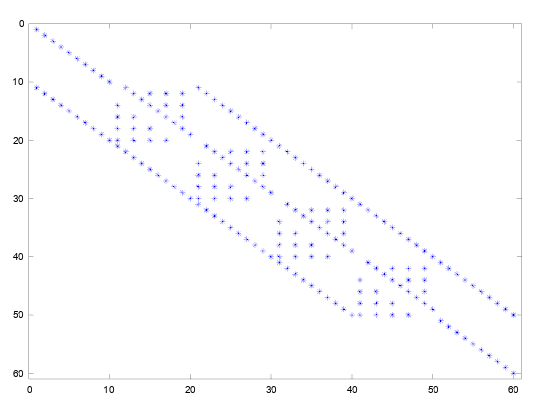
\includegraphics[width=\textwidth]{spy.png}
\caption{spy(A) for model 1 with N = M = 5}
\label{fig:spy}
\end{figure}

\subsection*{Model 2}



\section*{Perform numerical experiments with the BV-technique applied to both models. Illustrate your report with a couple of plots and tables}
\subsection*{Model 1}
In figure \ref{fig:spy}, the position of non-zero elements in our matrix $A$ can be seen.
We tested our method for $N = 10$ and $M = 100$. See figure \ref{fig:ucomp1} through \ref{fig:verr1} for a comparison of the exact solution and the values found with the BV-technique. Our implementation gives a reasonable estimation of $u$ and $v$, but a high accuracy is not achieved, especially for the high complexity of the BV-method. To obtain these results we had to solve a $2200\times2200$ ($2200 = 2*M*(N+1)$) linear system, which took about 30 seconds. During this calculation, Octave reported that our matrix $A$, was likely singular. We checked this by using $rank$, and found out that $A$ has $rank$ $2198$. After a while I realised that this is due to the characteristic of Leapfrog and our choice of $N$: $u$ on odd timesteps and $v$ on even timesteps are independent of $u$ on even timesteps and $v$ on odd timesteps. By choosing $N = 10$, our initial condition and final condition are both constraints on $u$ and $v$ in an even timestep, causing our matrix to be singular, and allowing invalid values for $u$ and $v$ on odd timesteps. After solving this problem by choosing $N$ odd, we have had far more accurate results and faster calculation;%TODO: explain properly
We have solved a system with $N = 9$ and $M = 100$, this took about $0.3$ seconds. The absolute error in $u$ improved by approximately a factor 3. See figure \ref{fig:uerr1small} and \ref{fig:verr1small}.
We have solved a system with $N = 201$ and $M = 200$, this took about $30$ seconds. See figure \ref{fig:uerr1big} and \ref{fig:verr1big} for the errors.

\begin{figure}
\centering
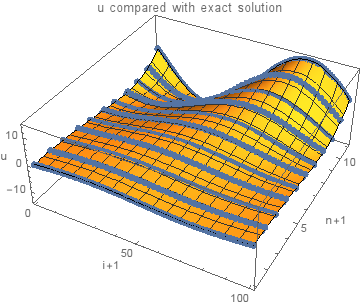
\includegraphics[width=0.6\textwidth]{uCompared.png}
\caption{In this plot the yellow surface represents the exact solution of $u$, while the blue lines are the results from the BV method for Model 1 with $N=10$ and $M=100$}
\label{fig:ucomp1}
\end{figure}

\begin{figure}
\centering
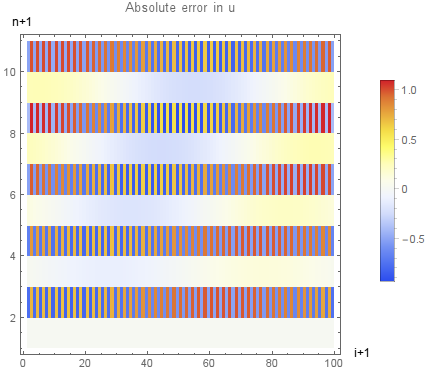
\includegraphics[width=0.6\textwidth]{errorUneat.png}
\caption{The absolute error in $u$ (Model 1 with $N=10$ and $M=100$)\\Notice that the error is low in even timesteps, but has higher amplitude (about $10\%$ relative error) and is alternating rapidly on odd timesteps.}
\label{fig:uerr1}
\end{figure}

\begin{figure}
\centering
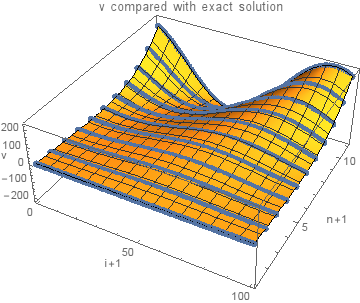
\includegraphics[width=0.6\textwidth]{vCompared.png}
\caption{In this plot the yellow surface represents the exact solution of $v$, while the blue lines are the results from the BV method for Model 1 with $N=10$ and $M=100$}
\label{fig:vcomp1}
\end{figure}

\begin{figure}
\centering
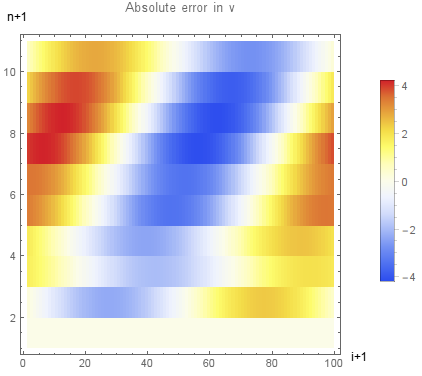
\includegraphics[width=0.6\textwidth]{errorVneat.png}
\caption{The absolute error in $v$ (Model 1 with $N=10$ and $M=100$)\\Notice that the amplitude of these errors is around 4, while the amplitude of $v$ is around 200. }
\label{fig:verr1}
\end{figure}

\begin{figure}
\centering
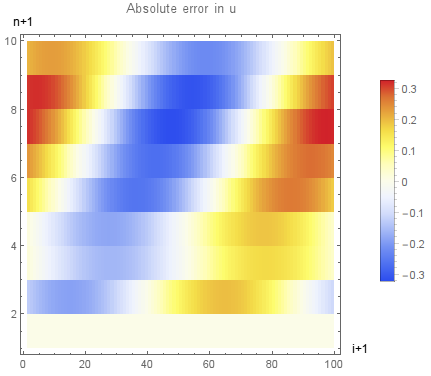
\includegraphics[width=0.6\textwidth]{errorUneat9x100.png}
\caption{The absolute error in $u$ (Model 1 with $N=9$ and $M=200$)\\Notice that the error is much smaller (approximately a factor 3) than that with $N=10$ and $M=200$.}
\label{fig:uerr1small}
\end{figure}

\begin{figure}
\centering
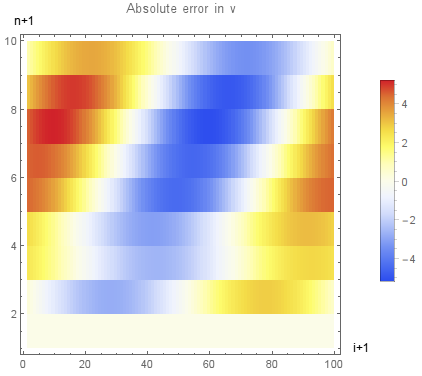
\includegraphics[width=0.6\textwidth]{errorVneat9x100.png}
\caption{The absolute error in $v$ (Model 1 with $N=9$ and $M=200$)\\Notice that the error is similar to that with $N=10$ and $M=200$.}
\label{fig:verr1small}
\end{figure}


\begin{figure}
\centering
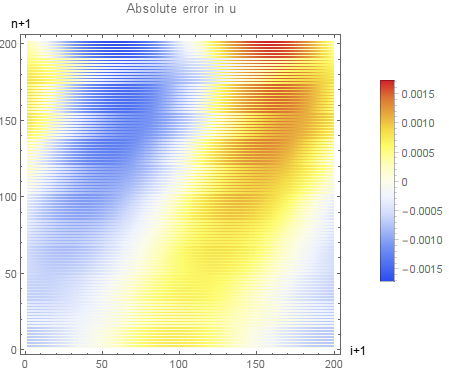
\includegraphics[width=0.6\textwidth]{errorUneat201x200.png}
\caption{The absolute error in $u$ (Model 1 with $N=201$ and $M=200$)\\Notice that the error is quite low.}
\label{fig:uerr1big}
\end{figure}

\begin{figure}
\centering
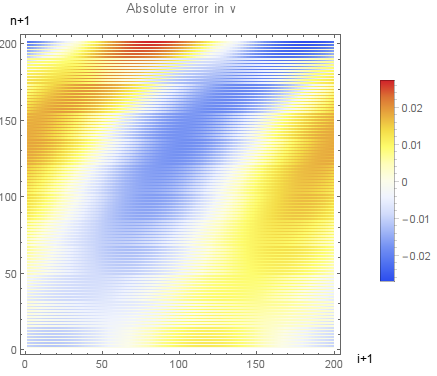
\includegraphics[width=0.6\textwidth]{errorVneat201x200.png}
\caption{The absolute error in $v$ (Model 1 with $N=201$ and $M=200$)\\Notice that the error is quite low.}
\label{fig:verr1big}
\end{figure}



\section*{Appendix A: BV-method implementation for model 1}
\lstinputlisting{bvmodel1.m}



\end{document}

